\documentclass[a4paper,twoside,12pt,chapterprefix=false,bibliography=totocnumbered,listof=flat]{scrbook}
\usepackage{lmodern}
\usepackage{amssymb,amsmath}
\usepackage{ifxetex,ifluatex}
\usepackage{fixltx2e} % provides \textsubscript
\ifnum 0\ifxetex 1\fi\ifluatex 1\fi=0 % if pdftex
  \usepackage[T1]{fontenc}
  \usepackage[utf8]{inputenc}
\else % if luatex or xelatex
  \ifxetex
    \usepackage{mathspec}
  \else
    \usepackage{fontspec}
  \fi
  \defaultfontfeatures{Ligatures=TeX,Scale=MatchLowercase}
\fi
% use upquote if available, for straight quotes in verbatim environments
\IfFileExists{upquote.sty}{\usepackage{upquote}}{}
% use microtype if available
\IfFileExists{microtype.sty}{%
\usepackage[]{microtype}
\UseMicrotypeSet[protrusion]{basicmath} % disable protrusion for tt fonts
}{}
\PassOptionsToPackage{hyphens}{url} % url is loaded by hyperref
\usepackage[unicode=true]{hyperref}
\hypersetup{
            pdftitle={Italian as non-native Language in Czechs and Slovak learners},
            pdfauthor={Marco Petolicchio},
            pdfborder={0 0 0},
            breaklinks=true}
\urlstyle{same}  % don't use monospace font for urls
\usepackage{natbib}
\bibliographystyle{apa}
\usepackage{longtable,booktabs}
% Fix footnotes in tables (requires footnote package)
\IfFileExists{footnote.sty}{\usepackage{footnote}\makesavenoteenv{long table}}{}
\usepackage{graphicx,grffile}
\makeatletter
\def\maxwidth{\ifdim\Gin@nat@width>\linewidth\linewidth\else\Gin@nat@width\fi}
\def\maxheight{\ifdim\Gin@nat@height>\textheight\textheight\else\Gin@nat@height\fi}
\makeatother
% Scale images if necessary, so that they will not overflow the page
% margins by default, and it is still possible to overwrite the defaults
% using explicit options in \includegraphics[width, height, ...]{}
\setkeys{Gin}{width=\maxwidth,height=\maxheight,keepaspectratio}
\IfFileExists{parskip.sty}{%
\usepackage{parskip}
}{% else
\setlength{\parindent}{0pt}
\setlength{\parskip}{6pt plus 2pt minus 1pt}
}
\setlength{\emergencystretch}{3em}  % prevent overfull lines
\providecommand{\tightlist}{%
  \setlength{\itemsep}{0pt}\setlength{\parskip}{0pt}}
\setcounter{secnumdepth}{5}
% Redefines (sub)paragraphs to behave more like sections
\ifx\paragraph\undefined\else
\let\oldparagraph\paragraph
\renewcommand{\paragraph}[1]{\oldparagraph{#1}\mbox{}}
\fi
\ifx\subparagraph\undefined\else
\let\oldsubparagraph\subparagraph
\renewcommand{\subparagraph}[1]{\oldsubparagraph{#1}\mbox{}}
\fi

% set default figure placement to htbp
\makeatletter
\def\fps@figure{htbp}
\makeatother

%\usepackage[a4paper,left=4.5cm, top=3.5cm, bottom=3.5cm, right=4.5cm, heightrounded, headsep=2em, footskip=11mm, vmarginratio=1:1]{geometry}
\usepackage[a4paper,margin=4cm, bindingoffset=1cm, heightrounded, headsep=2em, footskip=11mm, vmarginratio=1:1]{geometry}
\makeatletter
\DeclareOldFontCommand{\rm}{\normalfont\rmfamily}{\mathrm}
\DeclareOldFontCommand{\sf}{\normalfont\sffamily}{\mathsf}
\DeclareOldFontCommand{\tt}{\normalfont\ttfamily}{\mathtt}
\DeclareOldFontCommand{\bf}{\normalfont\bfseries}{\mathbf}
\DeclareOldFontCommand{\it}{\normalfont\itshape}{\mathit}
\DeclareOldFontCommand{\sl}{\normalfont\slshape}{\@nomath\sl}
\DeclareOldFontCommand{\sc}{\normalfont\scshape}{\@nomath\sc}
\makeatother




\usepackage{fontspec}

\usepackage{ifluatex}

\usepackage{microtype}



\setmainfont[Numbers=Lowercase]{IBMPlexSerif}
\setsansfont[Numbers=Lowercase]{IBMPlexSans}
\setmonofont[Numbers=Lowercase]{IBMPlexMono}


\usepackage[english]{babel}

\usepackage[all]{nowidow}

\usepackage[usenames, dvipsnames]{color}
\definecolor{upol-dGrey}{rgb}{0.36470588235,0.36862745098,0.37647058823}
\definecolor{upol-lGrey}{rgb}{0.8,0.8,0.8}
\definecolor{upol-brandBlue}{rgb}{0,0.43529411764,0.67843137254}


\usepackage{xcolor}
\usepackage{graphicx}
\definecolor{titlepagecolor}{cmyk}{1,.38,0,.15} %C100 M38 Y0 K15
\definecolor{namecolor}{cmyk}{0, 0, 0, .0980} 
\usepackage{textcase}


\usepackage{setspace}

\makeatletter\let\Title\@title\makeatother
%\makeatletter\let\Author\@author\makeatother



\usepackage{sectsty}
\allsectionsfont{\color{upol-dGrey}\sffamily}
\chapterfont{\color{upol-dGrey}\raggedleft\thispagestyle{empty}}





\usepackage{floatrow}
\floatsetup[table]{font=sf}
\floatsetup[figure]{font=sf}
\floatsetup[tikzpicture]{font=sf}

\usepackage[font={color=upol-dGrey}, labelfont={color=upol-dGrey}]{caption}



\makeatletter
\def\verbatim@font{\linespread{1}\footnotesize\ttfamily}
\makeatother



\makeatletter
\renewenvironment{figure}[1][\fps@figure]{
  \edef\@tempa{\noexpand\@float{figure}[#1]} 
  \@tempa
  \sffamily
}{
  \end@float
}
\renewenvironment{table}[1][\fps@table]{
  \edef\@tempa{\noexpand\@float{table}[#1]} 
  \@tempa
  \sffamily
  \footnotesize
}{
  \end@float
}
\makeatother

\usepackage{tabularx}
\usepackage{amsfonts}
\usepackage{booktabs}
\usepackage{siunitx}
\usepackage{fancyhdr}

\usepackage{lipsum, kantlipsum} % just for testing

\pagestyle{fancy}
\fancyhf{}
\fancyhead[LE,RO]{\thepage}
\fancyhead[RE]{\footnotesize\nouppercase{\leftmark}}
\fancyhead[LO]{\footnotesize\nouppercase{\rightmark}}
\setlength{\headheight}{14.5pt} % as requested by fan
\renewcommand{\headrulewidth}{0pt}

\renewcommand{\chaptermark}[1]{\markboth{\thechapter \ . \  #1}{}}
\renewcommand{\sectionmark}[1]{\markright{\thesection \ \ #1}{}}





%\setcounter{secnumdepth}{5}
%\setsecnumdepth{subsubsection}
%\maxtocdepth{subsubsection}


\setlength{\skip\footins}{3em}
\renewcommand\footnoterule{{\hrule height 0pt}} % a long blue line



\usepackage{colortbl}
\arrayrulecolor{gray}







\usepackage{booktabs}

\usepackage{pdfpages}






%Options: Sonny, Lenny, Glenn, Conny, Rejne, Bjarne, Bjornstrup
\usepackage[Bjornstrup]{fncychap}
%\renewcommand{\CNoV}{\raggedleft\sffamily\selectfont\HUGE}
  \ChNumVar{\Huge\sffamily\selectfont}
\renewcommand{\DOCH}{%
   \settowidth{\py}{\CNoV\thechapter}
  \addtolength{\py}{1em}      % Amount of space by which the
%                                % number is shifted right
   \fboxsep=0pt%
   \colorbox[gray]{.85}{\rule{0pt}{50pt}\parbox[b]{\textwidth}{\hfill}}%
   \kern-\py\raise20pt%
   \hbox{\color{gray}\CNoV\thechapter}\\%
}

\makeatletter
\renewcommand*{\@makechapterhead}[1]{%
  \vspace*{0\p@}%
  {\parindent \z@ \raggedright \normalfont
    \ifnum \c@secnumdepth >\m@ne
      \if@mainmatter%%%%% Fix for frontmatter, mainmatter, and backmatter 040920
        \DOCH
      \fi
    \fi
    \interlinepenalty\@M
    \if@mainmatter%%%%% Fix for frontmatter, mainmatter, and backmatter 060424
      \DOTI{#1}%
    \else%
      \DOTIS{#1}%
    \fi
  }}
% For the case \chapter*:
\renewcommand*{\@makeschapterhead}[1]{%
  \vspace*{10\p@}%
  {\parindent \z@ \raggedright
    \normalfont
    \interlinepenalty\@M
    \DOTIS{#1}
    \vskip 0\p@
  }}
\makeatother




\renewcommand*\chapterpagestyle{empty}




\usepackage{tikz,tikz-qtree}


\tikzstyle{every picture}+=[font=\sffamily]

\usepackage{listings}
\lstset{ %Formatting for code in appendix
	backgroundcolor = \color{gray},
	language=Python,
	basicstyle=\singlespacing\footnotesize\ttfamily\color{white},
	numbers=left,
	stepnumber=1,
	showstringspaces=true,
	tabsize=2,
	breaklines=true,
	breakatwhitespace=false,
	xleftmargin=3em,framexleftmargin=3em, numberstyle=\ttfamily,
}

\usepackage{datetime}

\let\oldmaketitle\maketitle
\AtBeginDocument{\let\maketitle\relax}




\usepackage{catchfilebetweentags}

\usepackage[autostyle]{csquotes}  
\usepackage{enumerate}


\makeatletter
\newcommand\HUGE{\@setfontsize\Huge{36}{48}} 
\makeatother

\usepackage{tikz}
\usepackage{pgfplots}


\usepackage{gb4e}
\noautomath

\setlength{\parskip}{1em}
\setlength{\parindent}{2em}

\usepackage[modulo]{lineno}

\preto{\chapter}{\resetlinenumber}
\linenumbers


\makeatletter
\newenvironment{chapquote}[2][2em]
  {\setlength{\@tempdima}{#1}%
   \def\chapquote@author{#2}%
   \parshape 1 \@tempdima \dimexpr\textwidth-2\@tempdima\relax%
   \itshape}
  {\par\normalfont\hfill--\ \chapquote@author\hspace*{\@tempdima}\par\vspace{4em}}
\makeatother

\frontmatter

\title{Italian as non-native Language in Czechs and Slovak learners}
\providecommand{\subtitle}[1]{}
\subtitle{From the development of a learner corpus towards a theoretical
investigation}
\author{Marco Petolicchio}
\date{2021-03-04}

\begin{document}
\maketitle

\makeatletter
\begin{titlepage}
\color{namecolor}

\pagecolor{titlepagecolor}

\noindent
\makebox[0pt][l]{\rule{1.4\textwidth}{1pt}}
\par

\noindent
\textbf{\sffamily{Palacký University}} \textcolor{namecolor}{\sffamily{ Olomouc}}\par \vskip\baselineskip 

\noindent\sffamily{Ph.D. Thesis in Italian Linguistics} \\
\noindent\sffamily{Dept. of Romance Languages, Faculty of Arts} \par\vskip\baselineskip

\vspace{2em}

\begin{flushleft}

\noindent
{\HUGE \sf \@title  \par}\vskip\baselineskip

\noindent
{\Large \sf \@subtitle \par} \vskip\baselineskip
\end{flushleft}

\noindent
{\large{\sffamily\MakeTextUppercase{\@author}}\par} 
\vspace{4em}
\par \vskip\baselineskip
\noindent
\noindent\sffamily{\textbf{Supervisors}}\par \vskip\baselineskip
\noindent
\sffamily{\MakeTextUppercase{Dr. Francesco Bianco, Ph.D.} \\ Palacký University · {Dept. of Romance Languages, Faculty of Arts} }\par \vskip\baselineskip

\vspace{3em}

 {\footnotesize   \ttfamily{draft : : \today   : :  \currenttime} \par}

\color{black}

\end{titlepage}
\makeatother
\nopagecolor% Use this to restore the color pages to white
\pagecolor{white}

{
\setcounter{tocdepth}{1}
\tableofcontents
}
\listoftables
\listoffigures
\chapter*{Preface}\label{preface}
\addcontentsline{toc}{chapter}{Preface}

\section*{Abstract}\label{abstract}
\addcontentsline{toc}{section}{Abstract}

The main topic of this doctoral dissertation is on the analysis of
syntactic structures in language acquisition, specifically in the domain
of Czech and Slovak learners which acquire the Italian language. In
particular, I will focus on the complex noun phrase subdomain, showing
the compositionality of the phrase structure and the hierarchical
fashion of this component. The analysis is casted in the
Minimalist-oriented framework of the Generative Grammar
\citep{chomsky1995, chomsky1998, chomsky2013, hcf2002} and its
application in the field of the second language acquisition
\citep{rothmanslabakova2017, slabakovalealliskin2014}.

The usage of an established computational ground to conduct the work,
where the data retrieved by fieldwork is stored in a coherent corpus
which easily permits to be queried and interpolated for the research
purposes, represents a standpoint for this research in its totality,
yielding for a data-based approach to the whole process. The annotation
schema of the data is standardized in order to adhere to the major point
of discussion into the discipline
\citep{clark2010, kueblerzinsmeinster2015, kurdi2016}, representing the
plus to furnish a data source which is independent to the merely
contingent purposes.

This research aims to offer a way to investigate how second language
acquisition can be seen grounding on a coherent set of data in terms of
annotation schema: it does insist either on the speculative questions
both on computational models involved.

\section*{Keywords}\label{keywords}
\addcontentsline{toc}{section}{Keywords}

Computational Linguistics; Syntax; Second Language Acquisition; Italian
L2; Corpus Linguistics.

\mainmatter

\chapter{Introduction}\label{introduction}

The main question of this thesis yields a twofold mindset that is not a
corollary of the research but represents the process in which the work
was conducted: how could I investigate a particular area of the language
faculty as language acquisition in a way which can gain from the usage
of the digital instruments in order to ground the theoretical analysis
on actual data?

The idea under this research moves across the motivation to investigate
over an empirically-grounded path the strategies shown by the learners
during the acquisition of second languages, using an established
coherent digital architecture. My task is twofold: on one side this
provides for the developing of a theoretically-grounded framework to
research in the fields of Second Language Acquisition (SLA), while on
the other this necessitates to develop a linguistic corpus which
collects into a coherent fashion a set of data that represent some
spotted linguistic fact in order to give a transparent documentation of
the learning path. The usage of the modern tools in developing a
linguistic corpus yields for a fully documentable research path, in
which is possible to reconstruct the steps and the choices which
underlie its development, the methods used in the analysis, the
correctness of the outcomes. This kind of research is intimately
multidisciplinar in nature, embracing different approaches and areas of
interest: digital humanities, corpus and computational linguistics for
the development of the linguistic corpus, general and theoretical
linguistics, studies on SLA and interlanguage for the theoretical
analysis.

This introductive chapter collects a preliminary way to represent the
main areas of the research, the methods involved in the analysis and the
possible outcomes of such a way to conduct the work.

\section{Background for the thesis}\label{background-for-the-thesis}

Corpus Linguistics is a field of approaches developed during the last
decades in order to give an empirical support to the investigations on
language use and variation. It can offer strong support for analyzing
the systematics which underlies the variations among the language use,
yielding for empirical and quantitative methods.

\begin{quote}
In fact, at one level it can be regarded as primarily a methodological
approach:

\begin{itemize}
\tightlist
\item
  it is empirical, analyzing the actual patterns of use in natural
  texts;
\item
  it utilizes a large and principled collection of natural texts, known
  as a \enquote{corpus}, as the basis for analysis;
\item
  it makes extensive use of computers for analysis, using both automatic
  and interactive techniques;
\item
  it depends on both quantitative and qualitative analytical techniques
  \citep{biber1998}
\end{itemize}
\end{quote}

The main tenets of such a discipline still permit to obtain different
level of information starting from the texts and their annotations, to
result in a general picture of the language variation. A part of this is
due to a widespan documentation which overpasses the recognized
linguistic theories - under the \emph{corpus-driven} approach. On the
other, the \emph{corpus-based} approach permits to ground the hypothesis
on a real actual set of data constitutes by language use in an
empirically based way.

\subsection{Corpus-based approach: motivations for the
thesis}\label{corpus-based-approach-motivations-for-the-thesis}

While a strong opposition between the way to approach the corpora can be
fairly molded during the actual analysis of the data in a softer manner,
it can be useful to stand up and recognize those models to threat
linguistic data as a two different standpoints to keep in mind for the
different purposes they grow on:

\begin{itemize}
\item
  \textbf{Corpus-based}\\
  When a general theory on some linguistic fact is tested against a
  corpus in order to verify the hypotheses. This kind of approach is
  more \emph{deductive}, while it goes top-down, proceeding from a
  general statement (the theory) towards a specific environment (the
  corpus).
\item
  \textbf{Corpus-driven}\\
  Corpus-driven approach tends to proceed from the analysis of the
  partial specific pieces (the corpus), in order to result into a
  general picture (the theory). This method is more \emph{inductive},
  going bottom-up.
\end{itemize}

Different views were proposed to face or embrace the corpora in language
studies amongst the scholars. The first one is a well-known citation by
\href{https://en.wikipedia.org/wiki/Noam_Chomsky}{Noam Chomsky}, which
substantially regrets any importance to corpora for a theory-oriented
language modeling:

\begin{quote}
Any natural corpus will be skewed. Some sentences won't occur because
they are obvious, others because they are false, still others because
they are impolite. The corpus, if natural, will be so wildly skewed that
the description would be no more than a mere list. \citep[Chomsky 1962,
\emph{A transformational approach to syntax} in][]{togninibonelli2001}
\end{quote}

On the other hand,
\href{https://en.wikipedia.org/wiki/Charles_J._Fillmore}{Charles
Fillmore} recognizes a structural place to corpora usage into language
reflection:

\begin{quote}
I have two main observations to make. The first is that I don't think
there can be any corpora, however large, that contain information about
all of the areas of English lexicon and grammar that I want to explore;
all that I have seen are inadequate. The second observation is that
every corpus that I've had a chance to examine, however small, has
taught me facts that I couldn't imagine finding out about in any other
way. \citep{fillmore1992}
\end{quote}

As in Fillmore's quotation, it appears that the distinction between
deductive and inductive method cannot be really disentangled in some
part of the research planning, moreover in the case when the one which
is developing a corpus is the same that is going to write an analysis
based on: a simple scan of the data can yields for a purpose of a
general theory which needs to be refined on the real data in a more
euristic manner. In this sense, while a \emph{corpus-based} approach
aims to generalize a picture \emph{before} than the actual recognition
of the data and the dataset takes place, it can be possible to softener
a bit this difference amongst these models keeping in mind the
perspective of corpus-developing related issues.

In the subsequent parts of the thesis I will try to show how the way to
develop a linguistic corpus has a certain degree of influence for the
successive part of research activities, and how a purely
\emph{corpus-based} method could not be apply if the research is
conducted by the same person which started to collect the data.

\subsection{Learners corpora of Italian L2: an
overview}\label{learners-corpora-of-italian-l2-an-overview}

In this section I am going to summarize the most representative Italian
L2 learner corpora available online, including Czech-IT, which I have
co-founded since July, 2017. I will present all the relevant information
and discuss the central topics of the project in a dedicate part of the
thesis, while for now I list the most evaluable corpora for studying
Italian as 2nd language:

\begin{itemize}
\item
  \textbf{\href{http://www.valico.org/valico_b_CORPUS.html}{GranVALICO}}
  and \textbf{\href{http://www.valico.org/valico_CORPUS.html}{VALICO}}
  \citep{valico}\\
  Learner corpora provided by Turin University. They represent the most
  valuable sources of Italian L2 corpora. They are composed by written
  texts composed by the students which have the assignment to describe
  the vignettes provided by the teachers. The corpora are accessible
  online with an advanced search that permits to filter the data by
  different parameters (e.g.~learners' L1 and education, assignments
  etc.).
\item
  \textbf{\href{http://merlin-platform.eu}{MERLIN}} \citep{merlin}\\
  The MERLIN Corpus represents a wide-range multilingual documented
  resource which collects 2.286 texts written by learners of Czech,
  Italian and German. Started in 2012, the main objective is to show the
  different levels of acquiring languages by the usage of written texts,
  relying on the CEFR level schema on L2 acquisition. The Italian-L2
  subcorpus contains 813 texts.
\item
  \textbf{\href{http://parlaritaliano.it/index.php/en/data/653-corpus-lips}{LIPS}}
  \citep{lips}\\
  The corpus contains the transcriptions of more than 2000 audio files
  by CILS - Certificazione di Italiano come Lingua Straniera (CILS) at
  the Università per Stranieri of Siena between the years 1993--2006.
  With more than 700k of words divided in \emph{monologues} and
  \emph{dialogues} between the candidate and the examiner, it represents
  one of the biggest corpora of Italian L2. The corpus is POS annotated
  using the tool Treetagger \citep{schmid1994}.
\item
  \textbf{\href{http://czech-it.github.io}{Czech-IT}} \citep{czech-it}\\
  The Czech-IT corpus contains chat messages, emails, coversations,
  surveys and assignments by more than 70 Czech and Slovak learners of
  Italian language. Started in 2017, it is fully accessible online while
  the data acquisition continues. The whole dataset is fully
  interrogable by an interactive interface and released with a Creative
  Commons license; POS and automatic tagging are in tune.
\item
  \textbf{\href{http://www.parlaritaliano.it/index.php/it/corpora-di-parlato/662-corpus-italiano-scritto-l2}{Corpus
  Italiano scritto L2}} \citep{vogheraturco2010}\\
  The corpus retains 227 written texts by undergraduate students of
  different native languages, which study Italian as a foreign language
  for their courses at the University of Greenwich. Learners' L1 are:
  albanian, bosniac, chinese, french, greek, english, norwegian,
  portuguese, spanish, tigrinya.\\
  The type of texts are: \emph{descriptive}, \emph{narrative} and
  \emph{argumental}. The texts are syntactically annotated and the
  tagset is available in xml format.
\end{itemize}

\begin{longtable}[]{@{}llrrrr@{}}
\caption{Size of Italian L2 Corpora}\tabularnewline
\toprule
Corpus & L1 & Texts & Tokens & Lemma & Years\tabularnewline
\midrule
\endfirsthead
\toprule
Corpus & L1 & Texts & Tokens & Lemma & Years\tabularnewline
\midrule
\endhead
GranVALICO & Various & 4778 & 784217 & 13057 & 2002--2007\tabularnewline
VALICO & Various & 2502 & 382098 & 6935 &\tabularnewline
LIPS & Various & 2198 & \textgreater{} 700000 & &
1993--2006\tabularnewline
MERLIN & Various & 813 & & & 2012--?\tabularnewline
Czech-IT & cs,sk & 316 & 17064 & & 2017--present\tabularnewline
Corpus Italiano Scritto L2 & Various & 227 & 22931 & &
2010?\tabularnewline
\bottomrule
\end{longtable}

\section{Objectives of the thesis}\label{objectives-of-the-thesis}

The three main objectives of this thesis are methodological, empirical
and theoretical.

\begin{enumerate}
\def\labelenumi{\arabic{enumi}.}
\tightlist
\item
  \textbf{Methodological objectives}\\
  To address the decisions and the methods raised by the compilation,
  the storage and the design of a learner based corpus, exploring the
  effective procedures for retrieving the relevant features for the
  analysis;
\item
  \textbf{Empirical objectives}\\
  To explore the previous generalizations of the acquisitional path in
  SLA literature comparing with the amount of linguistic productions
  given by different learners;
\item
  \textbf{Theoretical objectives}\\
  To describe the features which are relevant for characterise the
  language variety effect and the place of interlanguage.
\end{enumerate}

\subsection{Methodological objectives}\label{methodological-objectives}

While usually seen as a sussidary tool for linguistic investigations,
corpus linguistics can be regarded with a certain degree of indipendence
by such aims \citep{sinclair2005, sinclairCarter2004}, and involves
highly specialized sectors for what concerns the planning, the
mantaining, the design and the scalability of the corpora.

The Czech-IT corpus is composed by different kind of texts in order to
exhibit the variation in language use across different communicative
situations:

\begin{itemize}
\tightlist
\item
  Email subcorpus for the (quasi-) bureaucratic and academic language;
\item
  SMS and other direct platforms for textual messaging for informal
  situations;
\item
  Spoken discourse analysis for spontaneous modality;
\item
  Online surveys created for obtaining auto-evaluation by learners about
  their acquisition: the tests are made by a certain amount of questions
  and tiny writing samples.
\end{itemize}

75 are the learners inserted in the corpus. Informations about the
learners concern the education level, the age group, the level of their
italian knowledge, and other known languages - while their real
identities are preserved by the assignment of an alpha-numeric ID.

\subsection{Empirical objectives}\label{empirical-objectives}

Amongst many scholar the role of the native language (L1) has been
raised as a factor of possible conditionation in the way which the
target language (L2) is acquired during the learning path: an emblematic
case is the \emph{transfer} of the knowledge about the structures of the
L1 to the target, revealing the intermediate steps of the acquisitional
path defined with the term \emph{interlanguage} \citep{selinker1972},
that we can refer as to \textbf{Interlanguage Hypothesis} (IlH).
Different from this hypothesis --which recognizes a central place to the
native language in the acquisitional path-- is the \textbf{Monitor
Model} \citep{krashen1981}, a multi-focal perspective on language
acquisition where different factors are described as involved in the
process and where the L1 could not represent that conditionation.

Since the last 20 years, a considerable part of linguistic activity is
involved in developing some sort of models to describe how the faculty
of language can work, in its biological \citep{hcf2002}, computational
\citep{fodor2001} and cognitive components in a highly interdisciplinary
environment. Studies on SLA is a fertile field, which relies on
comparative and contrastive analyses of linguistic phenomena, either
both from an applied view \citep{ellis1994} than by theoretically
grounded perspective focused on Generative framework (GenSLA)
\citep{guasti2002, hawkins2001, rothmanslabakova2017, sorace2011}. In
this sense appears that the adoption of a general picture in which
analysing the variation in grammar into a \emph{parametric} model
\citep{chomsky1995} can be suitable for long-standing researches on SLA
and interlanguage.

The dataset used in this thesis aims to display either the different
linguistic outcomes in a wide range of communicative situations by the
same learner, both than a sociolinguistic grained analysis where the
variety of educational or age range can show different linguistic
behaviors in the range of learners' variety.

\subsection{Theoretical objectives}\label{theoretical-objectives}

From a theoretical viewpoint, the research is inserted in the current
theories that rely on the hierarchical functioning of the language
faculty, for which the variation among languages are reconducted to a
parametrizing of choice amongst the languages
\citep{adger2013, chomsky1995, chomsky1998, chomsky2013, chomsky2015, rizzi2013},
which are structurally constant, despite of the wideness of the
linguistic variation:

\begin{quote}
We are concerned, then, with states of the language faculty, which we
understand to be some array of cognitive traits and capacities, a
particular component of the human mind/brain. The language faculty has
an initial state, genetically determined; in the normal course of
development it passes through a series of states in early childhood,
reaching a relatively stable steady state that undergoes little
subsequent change, apart from the lexicon. To a good first
approximation, the initial state appears to be uniform for the species.
\citep{chomsky1995}
\end{quote}

This view permits on one side to compare the syntactic structures in a
coherent and schematic way, while on the other it concentrates moreover
on the hierarchical fashion of the language faculty than on the linear
order displayed by the utterances \citep{kayne1994, moro2000}. In this
perspective is generally assumed that the hierarchical phrase structure
plays a central role in syntactic computation, while the
\emph{flattering} of such structures into a mono-dimensional workspace
is a matter of externalization constraints and interface conditions
(e.g.~the need to give an ordered array where every item of the sentence
is present at one time in order to be spelled out). I will summarize
this in a representational way with the usual tree-diagram in
Fig.\ref{fig:tree1}.

\begin{figure}

{\centering 
\includegraphics[width=0.7\linewidth]{phdThesis_files/figure-latex/tree1-1} 

}

\caption{Structural representation of a simple sentence}\label{fig:tree1}
\end{figure}

Given this way to proceed, that assures a coherent framework to compare
languages in a parametric way, the main theoretical question addressed
here concerns the relevance and the potential usage of this perspective
in the analysis of a dynamic system as during the acquisitional path and
the strategies raised up by learners during the various steps in the
interlanguage.

\section{Outline of the thesis}\label{outline-of-the-thesis}

The first year is dedicated to the setting-up of the corpus, with the
starting operations to acquire the data and elaborate a coherent way to
annotate the texts with a standard schema. During the second year the
corpus is planned to grow up for reach a significance level of
\textgreater{}15000 words in order to provide quantitative analyses.
Third and fourth year will be spent in developing the theoretical
analyses and refining the informatic architecture of the project,
evolving in a user-friendly and interrogable way to dispense the data.
The theoretical outcome constitues the main topic of the research.

\textbf{Chapter 2} introduces \ldots{}

\textbf{Chapter 3} introduces \ldots{}

\textbf{Chapter 4} introduces \ldots{}

\textbf{Chapter 5} introduces \ldots{}

\chapter{Evidences and theories in a linguistic
research}\label{evidences-and-theories-in-a-linguistic-research}

\begin{chapquote}{Aristotle, \textit{Metaphysics, Book VIII, 1045a.8–10}}
\par{Pántōn gàr hósa pleíō mérē ékhei kaì mḕ éstin hoĩon sōròs tò pãn.}\\ 
\par{\noindent The totality is not, as it were, a mere heap, but the whole is something besides the parts.}
\end{chapquote}

\noindent It seems that a certain grade of analysis, theories and
empirical collect of data do not follow the same path, while they strike
one against the other: on one side the theoretical generalizations can
involve or not a verification of the hypotheses on the actual data that
the researcher can handle with, on the other the work around the data
collection can still confined without a well-grounded theoretical
approach. Nevertheless, while it does not imply \emph{per sé} that a
theoretical approach can be regarded as the primary goal for a
scientific approach, also the opposite knows some problems. Defining a
neutral way in which data should be collected is not an easy matter, and
someone could certainly ask if there is at all some sort of
\emph{rawness} or \emph{neutrality} in data itself\footnote{Cfr. the
  \emph{Observer Paradox} as stated by William Labov: \enquote{To obtain
  data on the most systematic form of language (the vernacular), we must
  observe how people speak when they are not being observed}
  \citep[xvii]{labov1973}.}.

\section{Inductivism and deductivism in
linguistics}\label{inductivism-and-deductivism-in-linguistics}

The inductivist approach to research begins with observations in forms
of singular events: they borrow a singular context of the place, the
time, and the particular situation in which each observation is made,
while the analysis of the similarities between such events yields for
generalizations.

In order to attempt a logic basis for a research method, Aristotle
distinguishes the \emph{induction} (\emph{epagōgē}) as the way which
preceeds from the particular to the universal, and the \emph{deduction}
(\emph{syllogismos}):

\begin{quote}
L'osservazione della somiglianza {[}\ldots{}{]} è utile, poiché siamo
convinti di suscitar l'universale attraverso l'induzione sui casi
singoli, che risultano simili: non è invero facile indurre, quando non
si conoscono le somiglianze degli oggetti. {[}\ldots{}{]} quanto si
applica eventualmente ad uno degli oggetti simili, si applicherà allo
stesso modo anche ai rimanenti. Di conseguenza {[}\ldots{}{]} quanto si
applica eventualmente ad essi si applichi allo stesso modo anche
all'oggetto della discussione \citep[ \emph{Topici}
1.18.108b]{aristoteleOrganon}.
\end{quote}

A well known example given by Bertrand Russell points out how the
inductivism approach can be a fallacy, making an expectation over
similar past events and applying these categories on the future:

\begin{quote}
Domestic animals expect food when they see the person who feeds them. We
know that all these rather crude expectations of uniformity are liable
to be misleading. The man who has fed the chicken every day throughout
its life at last wrings its neck instead, showing that more refined
views as to the uniformity of nature would have been useful to the
chicken \citep{russellProblems}.
\end{quote}

\subsection{Induction and empiricism}\label{induction-and-empiricism}

The inductive method proceeds bottom-up from a particular event to a
generalization of similar events into an uniform class of items,
commoned up by the property to display some analogies into their core
components. In this sense, the inductive way focuses on single,
individual phenomena as the starting point, collecting these into
subsets of similarities in order to attempt a rationale hypothesis which
can explain these similarities.

Basing from evidences as the starting point for critical investigation,
an inductive reasoning proceeds towards the elaboration of a general
rule that can expain the behaviour of different events in a similar
class. For achieving such kind of generalization, inductive hypotheses
rely on the principle which falls under the definition
\enquote{uniformity of nature}

\subsection{Deduction}\label{deduction}

\subsection{The role of empirical
data}\label{the-role-of-empirical-data}

\section{A theoretic framework to analyze the
data}\label{a-theoretic-framework-to-analyze-the-data}

\chapter{Moving the research into the digital
space}\label{moving-the-research-into-the-digital-space}

\section{Defining the kind of data}\label{defining-the-kind-of-data}

\section{Elaborating a corpus}\label{elaborating-a-corpus}

\chapter{An overview of the second language
acquisition}\label{an-overview-of-the-second-language-acquisition}

\chapter{Case study I}\label{case-study-i}

\chapter{Case Study II}\label{case-study-ii}

\chapter{Case study III}\label{case-study-iii}

\chapter{Conclusive remarks}\label{conclusive-remarks}

\backmatter

\chapter{Backmatter}\label{backmatter}

\section{Colophon}\label{colophon}

This document is typeset with LaTeX using a custom template based on
KOMA-script SCRBOOK class. The layout is based on a standard A4 paper
(210 x 297mm), with 40mm margins and 10mm of binding offset.

The typesetting software used the XeTeX engine and the text is set in
the open source IBM Plex font family -- in Serif, Sans Serif and
Monospace variants.

\section{Credits}\label{credits}

This project is constituted by files written in Markdown syntax and
exported either as a standalone website both as printer-ready product.
This is due to the awesome work of the people behind different
libraries:

\begin{itemize}
\tightlist
\item
  \href{https://bookdown.org}{Pandoc}
\item
  \href{https://bookdown.org}{Bookdown}
\item
  \href{https://bookdown.org}{RMarkdown} and
  \href{https://bookdown.org}{R} environment.
\end{itemize}

As well, for the computational infrastructure, some tools have been
used:

\begin{itemize}
\tightlist
\item
  \href{https://bookdown.org}{NLTK}
\item
  UDPIPE
\item
  SciPY
\end{itemize}

\section{About the author}\label{about-the-author}

I am a Graduate Researcher involved in a Ph.D.~Program in Italian
Linguistics at the Department of Romance Studies in the Faculty of
Philosophy at Palacky University in Olomouc, Czech Republic.

My interests span across digital humanities, syntax theories and
computational linguistics.

Feel free to write me at
\href{mailto:marco.petolicchio@gmail.com}{\nolinkurl{marco.petolicchio@gmail.com}}
or visit \href{http://marcopetolicchio.com}{marcopetolicchio.com} for
the detailed contact list.

\section{Progress in the repository}\label{progress-in-the-repository}

This graph represents the addition and deletion amount in the files of
the project in function of time.

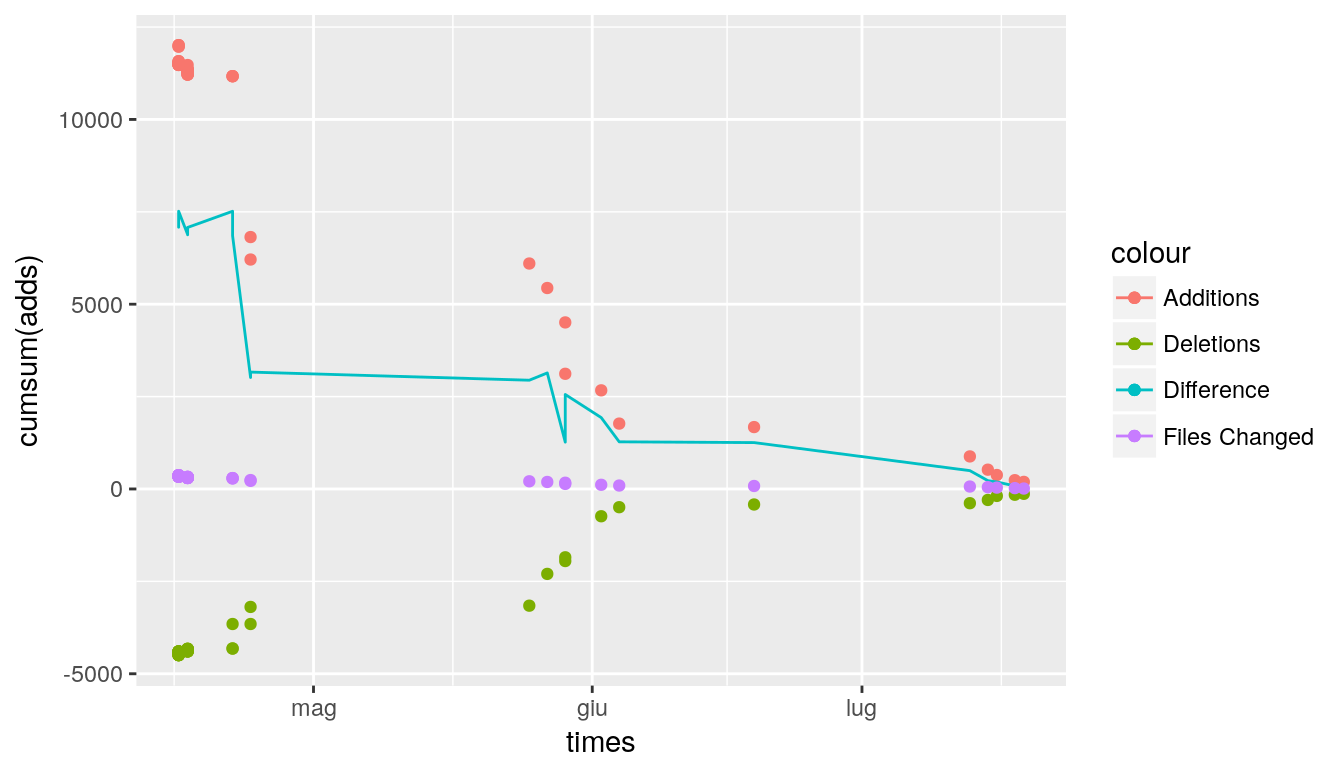
\includegraphics{phdThesis_files/figure-latex/unnamed-chunk-3-1.pdf}

\bibliography{bibliography.bib}

\end{document}
